\documentclass[letterpaper,final,12pt,reqno]{amsart}

\usepackage[total={6.3in,9.2in},top=1.1in,left=1.1in]{geometry}

\usepackage{times,bm,bbm,empheq,fancyvrb,graphicx}
\usepackage[dvipsnames]{xcolor}
\usepackage{longtable}
\usepackage{booktabs}

\usepackage[within=section]{newfloat}

\usepackage{tikz}
\usetikzlibrary{decorations.pathreplacing}

\usepackage[kw]{pseudo}
\pseudoset{left-margin=15mm,topsep=5mm,idfont=\texttt}

% hyperref should be the last package we load
\usepackage[pdftex,
colorlinks=true,
plainpages=false, % only if colorlinks=true
linkcolor=blue,   % ...
citecolor=Red,    % ...
urlcolor=black    % ...
]{hyperref}

\renewcommand{\baselinestretch}{1.05}

\allowdisplaybreaks[1]  % allow display breaks in align environments, if they avoid major underfulls

\newtheoremstyle{claim}% name
  {5pt}% space above
  {5pt}% space below
  {\itshape}% body font
  {}% indent amount
  {\itshape}% theorem head font
  {.}% punctuation after theorem head
  {.5em}% space after theorem head
  {\thmname{#1}\thmnumber{ #2}\thmnote{ (#3)}}% theorem head spec
\theoremstyle{claim}
\newtheorem{theorem}{Theorem}
\newtheorem{lemma}{Lemma}

\newcommand{\eps}{\epsilon}
\newcommand{\RR}{\mathbb{R}}

\newcommand{\grad}{\nabla}
\newcommand{\Div}{\nabla\cdot}
\newcommand{\trace}{\operatorname{tr}}

\newcommand{\hbn}{\hat{\mathbf{n}}}

\newcommand{\bb}{\mathbf{b}}
\newcommand{\be}{\mathbf{e}}
\newcommand{\bbf}{\mathbf{f}}
\newcommand{\bg}{\mathbf{g}}
\newcommand{\bn}{\mathbf{n}}
\newcommand{\br}{\mathbf{r}}
\newcommand{\bu}{\mathbf{u}}
\newcommand{\bv}{\mathbf{v}}
\newcommand{\bw}{\mathbf{w}}
\newcommand{\bx}{\mathbf{x}}

\newcommand{\bF}{\mathbf{F}}
\newcommand{\bV}{\mathbf{V}}
\newcommand{\bX}{\mathbf{X}}

\newcommand{\bxi}{\bm{\xi}}

\newcommand{\bzero}{\bm{0}}

\newcommand{\rhoi}{\rho_{\text{i}}}

\newcommand{\ip}[2]{\left(#1,#2\right)}

\newcommand{\mR}{R^{\bm{\oplus}}}
\newcommand{\iR}{R^{\bullet}}

\newcommand{\nn}{{\text{n}}}
\newcommand{\pp}{{\text{p}}}
\newcommand{\qq}{{\text{q}}}
\newcommand{\rr}{{\text{r}}}

\newcommand{\bus}{\bu|_s}

% norm |||x|||
\newcommand{\vertiii}[1]{{\left\vert\kern-0.25ex\left\vert\kern-0.25ex\left\vert #1 \right\vert\kern-0.25ex\right\vert\kern-0.25ex\right\vert}}

% numbering
\setcounter{tocdepth}{3}
\makeatletter
\def\l@subsection{\@tocline{2}{0pt}{4pc}{5pc}{}}
\makeatother

\numberwithin{equation}{section}
\numberwithin{figure}{section}
\numberwithin{table}{section}
\numberwithin{theorem}{section}

\DeclareFloatingEnvironment[name=Pseudocode]{pcode}

\begin{document}
\title[Multilevel computation of glacier geometry from Stokes dynamics]{Multilevel computation of glacier geometry \\ from Stokes dynamics}

\author{Ed Bueler}

\author{Lawrence Mitchell}

\begin{abstract} FIXME MCD for steady and evolving geometry with Glen-Stokes dynamics
\end{abstract}

\maketitle

%\tableofcontents

\thispagestyle{empty}
%\bigskip

\section{Introduction} \label{sec:intro}

FIXME MCD = multilevel constraint decomposition, a multigrid \cite{Trottenbergetal2001} method basically by \cite{Tai2003} for obstacle problems; see \cite{Bueler2022};  obstacle problem view first extended to Stokes by \cite{WirbelJarosch2020};  The computations in this paper use the Python FE library Firedrake \cite{Rathgeberetal2016}, which applies an embedded domain language \cite{Alnaesetal2014} to convert weak forms into discrete equations which are solved in parallel using the PETSc \cite{Balayetal2020} library.


\section{The steady ice geometry problem} \label{sec:stokesgeometry}

The standard model for determining the geometry of glaciers is based in part upon a dynamical description of ice flow, namely a shear-thinning version of the Stokes equations.  This Glen-Stokes ice-dynamics model can only determine the free-surface glacier geometry when it is combined with the surface kinematical equation (SKE) and a climate input, namely the balance of the rates of accumulation of snow and of ablation, i.e.~melting and runoff.  In this section we state the strong form of the resulting ``coupled'' glacier geometry model in the steady-state case, which we call the steady ice geometry problem (SIGP).  The emphasis here is on the complementarity-problem nature of the SIGP, which is often not explicit in the glaciers literature (e.g.~as observed by \cite{SchoofHewitt2013}).  We then define its weak form, noting along the way several unknown aspects of the theory.  Section \ref{sec:evolution} gives the straightfoward extension of the steady case to a time-discretized evolving-geometry model, the implicit ice geometry problem (IIGP).

The SIGP is defined on a fixed, bounded map-plane region $\Omega \subset \RR^d$ for $d=1,2$ (Figure \ref{fig:stokesdomain}).  The coordinates on $\Omega$ are denoted as $x$ when $d=1$ and $x,y$ when $d=2$.  On $\Omega$ we assume that a climatic mass balance (CMB) \cite{Cogleyetal2011} function $a(x,y)$ is defined at every point, whether or not ice is present at that location.  In ice-free areas this function is the ``potential'' CMB, namely the annual balance of snow accumulation and melt if ice were present, e.g.~as computed by energy balance in a climate or weather model.  Here we assume $a$ has units of ice thickness per time, compatible with our assumption of constant ice density (below).  Next we assume there is a bed elevation function $b(x,y)$ defined everywhere on $\Omega$, which determines the topography upon which the glacier sits.  The functions $a$ and $b$ are the data (inputs) of the SIGP.

\begin{figure}[t]
\begin{center}
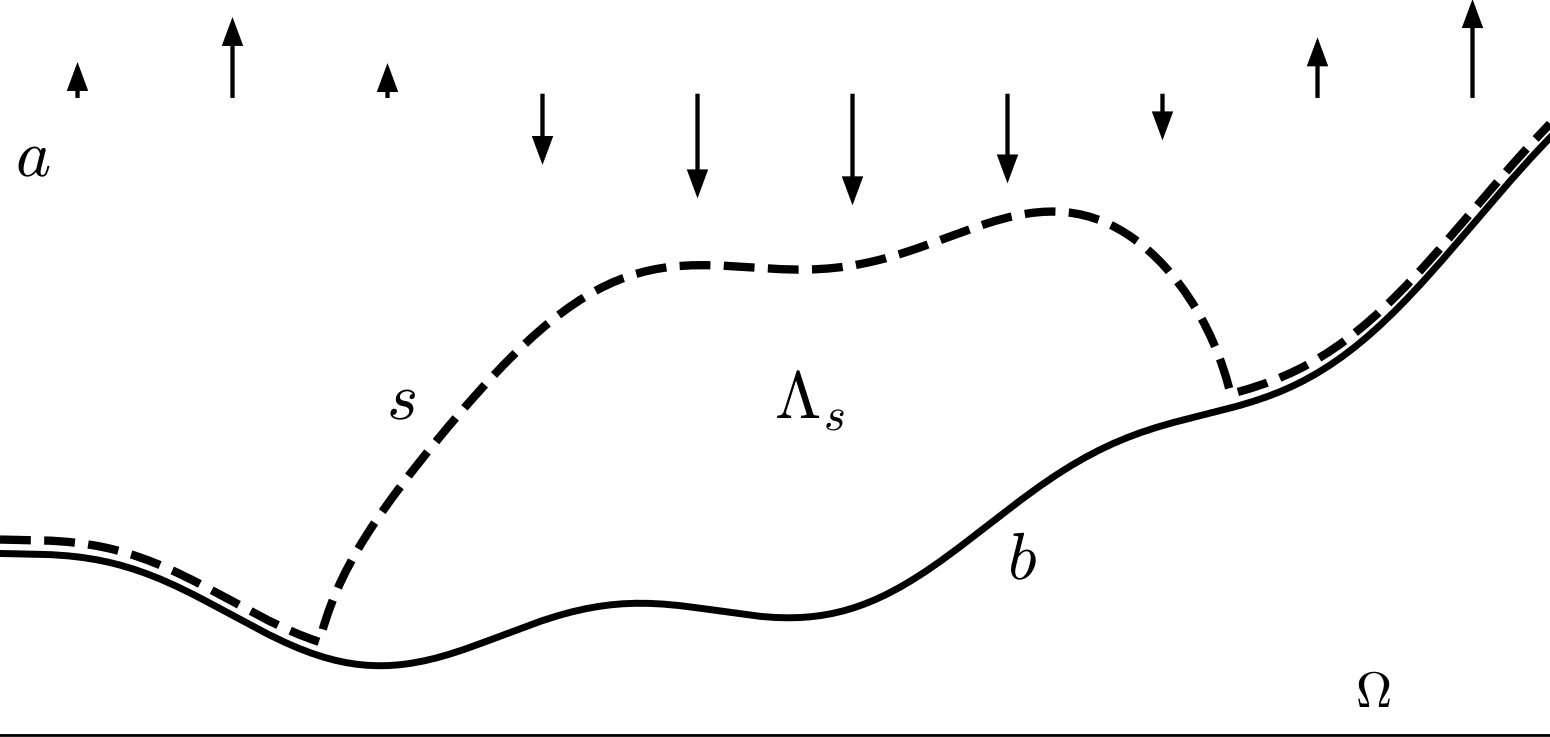
\includegraphics[width=0.7\textwidth]{genfigs/stokesdomain.pdf}
\end{center}
\caption{In the SIGP the CMB $a$ (arrows; down for accumulation) and bed elevation $b$ (solid) are given data on a map-plane region $\Omega \subset \RR^d$.  The solution includes a surface elevation $s$ (dashed) on $\Omega$, such that $s\ge b$, plus the ice velocity $\bu$ and pressure $p$ on the icy domain $\Lambda_s = \{b < z < s\} \subset \RR^{d+1}$.}
\label{fig:stokesdomain}
\end{figure}

The Glen-Stokes dynamical model, the so-called stress balance, only applies in the icy domain in $\RR^{d+1}$.  We make a strong, but common \cite[for example]{IsaacStadlerGhattas2015,Jouvetetal2008,Lengetal2012,WirbelJarosch2020} assumption this this icy domain has a well-defined upper surface elevation, a function $s(x,y)$.  That is, we assume there are \emph{no overhangs}, and that the under-side of the ice is in contact with the bed $b$.  We then define $s$ everywhere in $\Omega$ by extending with $s=b$ where ice is absent, thus $s\ge b$ applies on all of $\Omega$.  Note that $s$ is part of the model solution; it is not given data.

However, as a consequence of the no-overhangs assumption, the SIGP as described here is likely not to be well-posed because of an issue at the ice margin.  There may be no steady state because the fluid in the vicinity of a steep ice margin, especially on a steep bed feature, ``wants'' to generate an overhang, violating the assumption that the function $s$ is well-defined.  Furthermore the same concern applies to each time step of an evolving model; overhangs can develop at the margin.  Because overhangs are small features in large glaciers and ice sheets, most modeling literature ignores this possibility and assumes well-defined surface elevation and thickness \cite{Jouvetetal2008,Lengetal2012,WirbelJarosch2020}.  Exceptions \cite{PralongFunk2005} and \cite{Jouvetetal2011} provide a continuum model in which ice-cliff calving occurs via a damage variable and a stress-fracture failure criterion, and such a model might explain how (essentially) well-defined surface elevation and thickness could arise in a well-posed model.  However, such a model is a nontrivial extension of the above equations, and though marginal cliffs may exist in our model (Section \ref{sec:fe}), overhangs are never allowed herein.

Based on a well-defined upper surface, the icy domain is the open set
\begin{equation}
\Lambda_s = \{(x,y,z)\,|\,(x,y) \in \Omega \,\text{ and }\, b(x,y) < z < s(x,y)\}  \subset \RR^{d+1}, \label{eq:lambdas}
\end{equation}
where $z$ is vertically-upward.  (Coordinates are denote $(x,z)$ on $\Lambda_s$ when $d=1$.)  The domain $\Lambda_s$ has the topology of the product of an open subset of $\Omega$ and an interval, and we will approximate it using an extruded mesh (Section \ref{sec:fe}).  Again note $\Lambda_s$ is part of the solution.

We model the ice as an incompressible, very-viscous \cite{Acheson1990}, non-Newtonian fluid subject to Glen's shear-thinning flow law \cite{GreveBlatter2009}; see also \cite[Chapter 1]{FowlerNg2021}.  Allowing any Glen exponent $\nn\ge 1$, the equations inside $\Lambda_s$ are
\begin{align}
- \nabla \cdot \tau + \nabla p &= \rhoi \bg &&\text{\emph{stress balance}} \label{eq:forcebalance} \\
\nabla \cdot \bu &= 0 &&\text{\emph{incompressibility}} \label{eq:incompressible} \\
\tau &= B_\nn |D\bu|^{(1/\nn) - 1} D\bu  &&\text{\emph{flow law}} \label{eq:viscflowlaw}
\end{align}
The solution fields here are the velocity $\bu$, pressure $p$, and deviatoric stress $\tau$.  Equations \eqref{eq:forcebalance} and \eqref{eq:viscflowlaw} form the momentum conservation (stress balance) model, while \eqref{eq:incompressible} follows from constant density and mass conservation.

Regarding tensors and their notation, recall that the (Cauchy) stress tensor $\sigma$ decomposes into the deviatoric part $\tau$ minus the pressure, i.e.~$\sigma = \tau - p\,I$, so equation \eqref{eq:forcebalance} simply says $-\Div \sigma = \rhoi \bg$.  The strain rate tensor $D\bu$ is the symmetric part of $\grad \bu$, $D\bu = \frac{1}{2} \left(\grad\bu + \grad\bu^\top\right)$, and the tensor norm used in \eqref{eq:viscflowlaw} satisfies $|D\bu|^2 = \frac{1}{2} (D\bu)_{ij} (D\bu)_{ij}$.  Because $D\bu$ is symmetric, and because it has trace zero by equation \eqref{eq:incompressible}, i.e.~$\trace(D\bu)=\nabla \cdot \bu = 0$, equation \eqref{eq:viscflowlaw} then implies that $\tau$ is also symmetric with trace zero, thus that $p=-(d+1)^{-1} \trace \sigma$.

In computations we will use constants $\nn=3$, ice density $\rhoi=910 \,\text{kg}\,\text{m}^{-3}$ \cite{Huybrechtsetal1996}, and gravity $\bg=\left<0,0,-g\right>$, with $g=9.81\,\text{m}\,\text{s}^{-2}$.  The ice hardness $B_\nn$ is a constant because we assume isothermal conditions \cite{GreveBlatter2009}, with the value $B_3=6.8082\times 10^7\,\text{Pa}\,\text{s}^{1/3}$ \cite{Huybrechtsetal1996} used in computations.

For the $\nn=1$ (Newtonian) Stokes equations one would write \eqref{eq:viscflowlaw} as $\tau = 2\nu D\bu$ with viscosity $\nu>0$, but exponents $\nn>1$ imply an effective viscosity function of $|D\bu|$.  This would be singular in the limit of small strain rates, and so, motivated by the actual finite viscosity of glacier ice \cite{GreveBlatter2009}, we define the regularized effective viscosity using $\eps>0$,
\begin{equation}
\nu_\eps = \frac{1}{2} B_\nn \left(|D\bu|^2 + \eps\, D_0^2\right)^{(\pp-2)/2}, \label{eq:regeffvisc}
\end{equation}
where $\pp=(1/\nn)+1$, with $\pp=4/3$ in computations.  The constant $D_0$ defines a strain-rate scale for glacier flow; values $D_0 = 1 \,\text{a}^{-1}$ and $\eps = 10^{-4}$ are used in computations.

Our SIGP model uses dynamic boundary conditions for isolated, grounded, and non-sliding glaciers.  (Floating and sliding cases are topics for additional research.)  In addition to the already-stated assumption that the top and bottom boundaries of $\Lambda_s$ can be identified, we further assume these surfaces have well-defined tangents.  On the base we impose no slip:
\begin{equation}
\bu = \bzero  \qquad\qquad \text{\emph{base} } \Gamma_0. \label{eq:basebc}
\end{equation}
On the other sub-aerial surfaces we set a condition of zero applied stress,
\begin{equation}
\left(2 \nu_\eps D\bu - pI\right) \bn = \bzero  \qquad \qquad \text{\emph{top and cliffs (if present)}} \label{eq:topbc}
\end{equation}
where $\bn$ is any normal to $\overline{\partial} \Lambda$.  (A nonzero atmospheric pressure at the surface is straightforward to apply if desired.)  Note that the ice flow extends in the horizontal direction until a free boundary at the glacier margin is reached, but that $\grad s$ may become singular there.

The simultaneous determination of $\Lambda_s$ and $(\bu,p)$ is the goal of the SIGP model.  However, the above equations make no reference to the climate input function $a$, so we need another ``equation'', one which is actually an inequality.  Noting that the surface elevation is already defined on all of $\Omega$, with $s=b$ off the ice, we set
\begin{equation}
\bn_s = \left<-s_x,-s_y,1\right> \label{eq:surfacenormal}
\end{equation}
as an (un-normalized) top-surface normal almost everywhere on $\Omega$.  Furthermore we extend the surface value of the velocity to all of $\Omega$:
\begin{equation}
\bus(x,y) = \begin{cases} \bu(x,y,s(x,y)), & s(x,y) > b(x,y), \\
                     \bzero, & \text{elsewhere}. \end{cases} \label{eq:surfacevelocity}
\end{equation}
A discontinuity of this function is allowed at the ice margin.

The steady-state surface kinematical equation (SKE) \cite[equation (5.21)]{GreveBlatter2009} is the needed additional aspect of mass conservation:
\begin{equation}
\bus \cdot \bn_s + a = 0 \qquad \text{\emph{on the ice}}. \label{eq:ske}
\end{equation}
Note that $a(x,y)$ is the \emph{vertical} ice thickness added per time, while some references use a distinct quantity, namely the thickness added perpendicularly to the ice surface, significantly different if $\grad s$ is large.

Though kinematical balance \eqref{eq:ske} applies only on the ice, $\bus \cdot \bn_s + a \le 0$ applies everywhere in $\Omega$ because $a$ is nonpositive in steady state in ice-free locations.  In fact, when combined with the constraint that $s\ge b$ everywhere on $\Omega$, SKE \eqref{eq:ske} is part of an infinite-dimensional nonlinear complementarity problem (NCP) \cite{Bueler2021conservation}.  An NCP on a finite-dimensional vector space $V=\RR^k$ combines the three statements
\begin{equation}
x\ge 0, \quad f(x)\ge 0, \quad x f(x)=0 \label{eq:ncp}
\end{equation}
for all $x\in V$, where $f:V\to V$ \cite{FacchineiPang2003}.

We may now state the strong form of the SIGP, as follows, by including all of the above conditions, and also by eliminating $\tau$ from \eqref{eq:forcebalance} and \eqref{eq:viscflowlaw}:
\begin{align}
s - b &\ge 0 && \text{on $\Omega$} \label{eq:strongform} \\
- \bu|_s \cdot \bn_s - a &\ge 0 && \text{\emph{same}} \notag \\
(s - b) (- \bu|_s \cdot \bn_s - a) &= 0 && \text{\emph{same}} \notag \\
- \nabla \cdot \left(2 \nu_\eps\, D\bu\right) + \nabla p - \rhoi \mathbf{g} &= \bzero && \text{on $\Lambda_s$} \notag \\
\nabla \cdot \bu &= 0 && \text{\emph{same}} \notag \\
\bu &= \bzero && \text{on $\Gamma_0$} \notag \\
\left(2 \nu_\eps D\bu - pI\right) \bn &= \bzero && \text{on $\partial \Lambda_s \setminus \Gamma_0$} \notag
\end{align}
(Definition \eqref{eq:regeffvisc} of $\nu_\eps$ is included.)  The first three statements in \eqref{eq:strongform} form the NCP, but this problem is coupled to the boundary value problem formed by the last four statements.

The solution of \eqref{eq:strongform} is a triple of functions $s(x,y)$, $\bu(x,y,z)$, $p(x,y,z)$ on $\Omega,\Lambda_s,\Lambda_s$, respectively.  However, as the domain on which $\bu,p$ are defined is only known via the solution, \eqref{eq:strongform} is at best an incomplete description.  The weak form in the next section, using a solution operator which maps $s$ to $\bu|_s$, will partially address this concern.

However, whether in strong or weak form, inequality-constrained system \eqref{eq:strongform} has a largely-unknown theory regarding well-posedness and solution regularity.  Certain well-posedness theory is known for the SIA version of this problem, with existence established by \cite{JouvetBueler2012}, including uniqueness in the flat bed case.

After stating the SIGP weak form next in Section \ref{sec:weakido}, in Sections \ref{sec:fe}--\ref{sec:results} we will construct and demonstrate a multilevel scheme for the problem.  As noted in Section \ref{sec:intro}, numerical solutions have traditionally applied explicit time-stepping, even when computing steady states, splitting the dynamics and the SKE into sub-steps and using truncation to address the NCP \cite[for example]{Jouvetetal2008,Lengetal2012}.  By contrast, the implicit time-stepping model in Section \ref{sec:evolution} avoids time-splitting and is unconditionally stable.


\section{The weak form using an ice dynamics operator} \label{sec:weakido}

The weak form of the fixed-geometry Glen-Stokes model for ice flow, which extends the linear Stokes weak form \cite{Elmanetal2014} to regularized power-law rheology, is relatively well-known \cite{IsaacStadlerGhattas2015,JouvetRappaz2011,Lengetal2012}, and we summarize it here, after which we address the weak form of the SIGP.

Denote by $W^{k,r}$ the Sobolev space \cite{Evans2010} of functions with $k$ derivatives which are $r$th-power integrable.  Suppose for the moment that $\Lambda \subset \RR^{d+1}$ is a fixed, bounded domain on which we prescribe a Dirchlet condition $\bu=0$ on some positive-measure portion of the boundary, and otherwise suppose the boundary is stress-free (Neumann boundary).  Let $\pp=(1/\nn)+1$ as in \eqref{eq:regeffvisc}, and $\qq=(1-\pp^{-1})^{-1}=\nn+1$ the conjugate exponent; $\pp=4/3$ and $\qq = 4$ if $\nn=3$.  Let $W_0^{1,\pp}(\Lambda)^{d+1}$ be the space of velocity functions, zero along the Dirichlet boundary, and let
\begin{equation}
\mathcal{M}_\Lambda = W_0^{1,\pp}(\Lambda)^{d+1} \times L^\qq(\Lambda)  \label{eq:mixed}
\end{equation}
be the (mixed) space of admissible velocity and pressure pairs.  The Glen-Stokes solution $(\bu,p) \in \mathcal{M}_\Lambda$ should satisfy the weak form
\begin{equation}
F_\Lambda(\bu,p)[\bv,q] = \int_\Lambda 2 \nu_\eps D\bu : D\bv - p \Div\bv - (\Div\bu) q - \rhoi \bg \cdot \bv\,d\bx = 0 \label{eq:glenstokesweak}
\end{equation}
for all $(\bv,q) \in \mathcal{M}_\Lambda$.

Jouvet and Rappaz \cite{JouvetRappaz2011} prove that this fixed-domain Glen-Stokes formulation is well-posed under the above assumptions if also the Neumann boundary of $\Lambda$ is $C^1$.  In particular they show \eqref{eq:glenstokesweak} is equivalent to minimization of a convex and coercive functional over the divergence-free subspace, but also that there is a unique pressure $p$.

However, we must go beyond the problem on predetermined ice geometry to solve the weak form of \eqref{eq:strongform}.  Again suppose $\Omega \subset \RR^d$ is a fixed map-plane domain with $C^1$ boundary, and that the bed elevation $b$ is in $W^{1,\qq}(\Omega)$.  The Sobolev space $W^{1,\qq}(\Omega)$ supports a linear trace operator which defines the symbol $|_{\partial \Omega}$ \cite[Section 5.5]{Evans2010}.  Let
\begin{equation}
\mathcal{K} = \{s \in W^{1,\qq}(\Omega) \,:\, s \ge b \, \text{ and } \, s\big|_{\partial\Omega} = b\big|_{\partial\Omega}\}  \label{eq:Kconstraintset}
\end{equation}
be the closed and convex set of admissible surface elevations of an isolated glacier or ice sheet.  From now on we also assume that $\nn>1$.  Because $\qq = \nn+1 > d$, each $s \in W^{1,\qq}(\Omega)$ is continuous \cite[Morrey's inequality, section 5.6.2]{Evans2010}, and so there are no cliffs in the $s$ geometry.  (Though it is not clear that the correct Sobolev space is identified in \eqref{eq:Kconstraintset}, the constraint is surely correct.  Existence for the simpler SIA model finds a power of the ice thickness, $u=(s-b)^{2q/(q-1)}$, in $\mathcal{K} = \{v \ge 0\} \subset W^{1,\qq}(\Omega)$ \cite{JouvetBueler2012}.)

Recalling definition \eqref{eq:lambdas}, we further suppose that
\begin{equation}
s\in \mathcal{K} \text{ defines an icy domain } \Lambda_s \text{ which has a $C^1$ upper surface.} \label{eq:quixotic}
\end{equation}
Assumption \eqref{eq:quixotic} would follow from a sufficiently-strong regularity result for the theory of the current paper, which we cannot offer.  In the SIA model the surface $s$ solves an elliptic equation, so it is smooth on $\{s>b\} \subset \Omega$ if $b$ is itself smooth \cite{JouvetBueler2012}.

We now define the ice dynamics operator (IDO), a map $\Phi$ which uses the trace of the velocity solution to the Glen-Stokes problem above (Figure \ref{fig:idoaction}).  For each surface elevation function $s \in \mathcal{K}$ the output $\Phi(s)$ is the negative normal component of the (unique) velocity solution $\bu$ of \eqref{eq:glenstokesweak} over the upper surface of $\Lambda_s$, but extended by zero to all of $\Omega$:
\begin{equation}
\Phi(s) = \begin{cases} - \bu|_s \cdot \bn_s, & s > b, \\
                        0, & \text{otherwise}. \end{cases} \label{eq:ido}
\end{equation}
Here $\bu|_s$ denotes a trace operator on $W^{1,\pp}(\Lambda_s)^{d+1}$; compare \eqref{eq:mixed}.  Note that $\Phi(s)$ is a scalar function on $\Omega$ which may jump or have other singularities at the glacier margin, but we will only need $\Phi(s)$ to be in the dual of $W^{1,\qq}(\Omega)$.

\begin{figure}[t]
\begin{center}
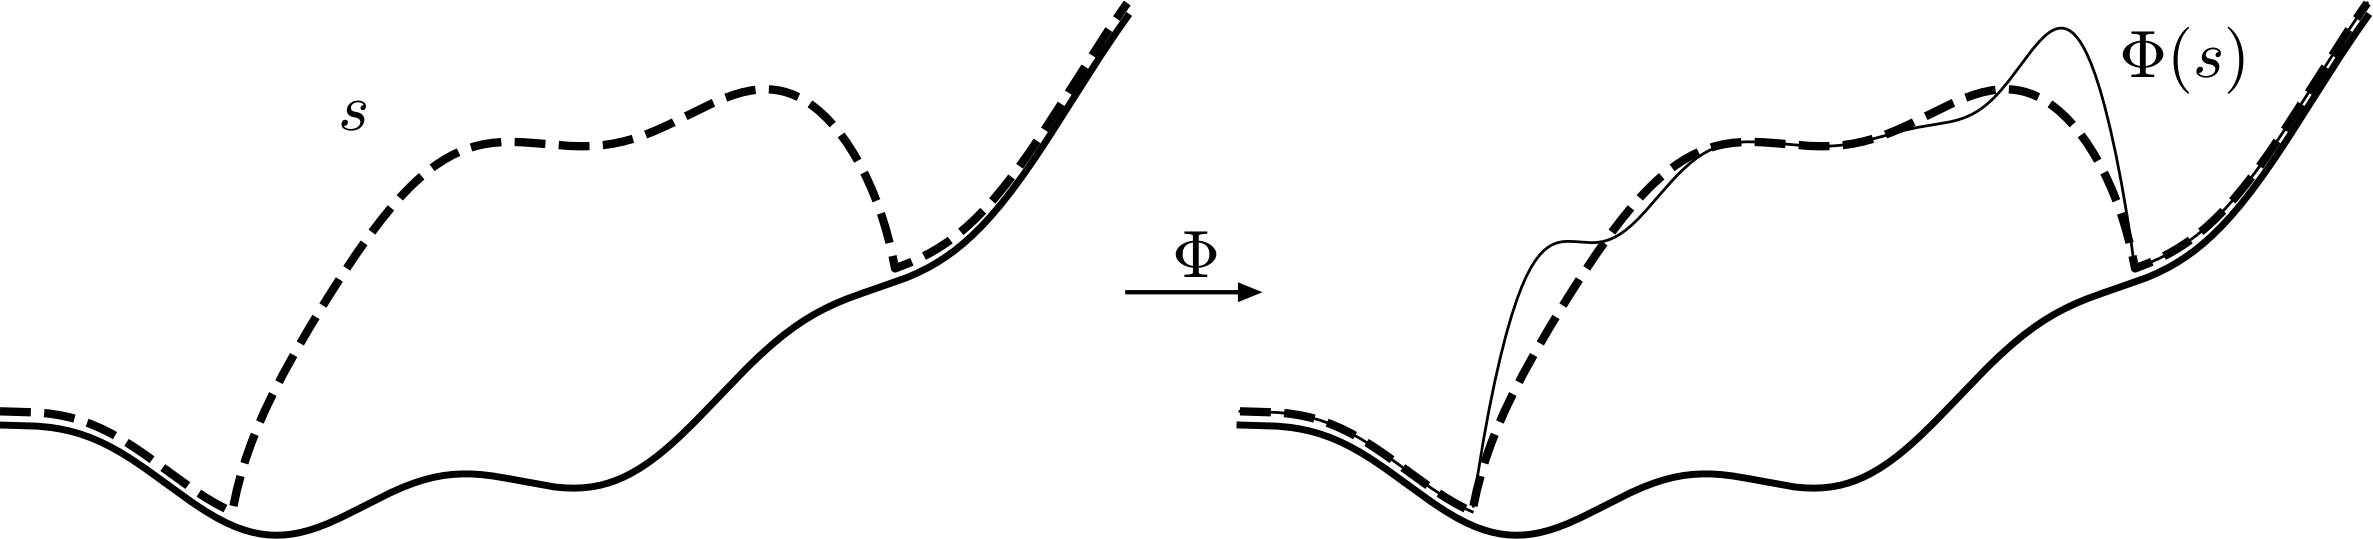
\includegraphics[width=\textwidth]{genfigs/idoaction.pdf}
\end{center}
\caption{The ice dynamics operator $\Phi$ maps the surface elevation $s$ (dashed) to the normal ice surface motion $\Phi(s)=- \bu|_s \cdot \bn_s$, equation \eqref{eq:ido}.  Both the input and output of $\Phi$ are defined on all of $\Omega$.}
\label{fig:idoaction}
\end{figure}

We believe that formula \eqref{eq:ido} defines a nonlinear operator $\Phi:\mathcal{K} \subset W^{1,\qq}(\Omega) \to (W^{1,\qq}(\Omega))^* = W^{-1,\pp}(\Omega)$.  This operator is \emph{expensive}; evaluating $\Phi(s)$ requires solving Glen-Stokes problem \eqref{eq:glenstokesweak} on $\Lambda_s \subset \RR^{d+1}$ defined in \eqref{eq:lambdas}.  Furthermore the operator is clearly \emph{nonlocal} because the solution $\bu$ is influenced everywhere by changes in the icy domain geometry.  In particular, if $\tilde s=s + r$ defines $\Lambda_{\tilde s} \supset \Lambda_s$, for $r\in C_c^\infty(\Omega)$ with $r\ge 0$ supported inside $\{s>b\}$, then the Stokes solutions are generically different everywhere both solutions are defined: $\tilde\bu - \bu \ne 0$ on all of $\Lambda_s$, including the trace on the upper surface.  Thus an FE discretization of $\Phi(s)$ will have a dense Jacobian matrix

By contrast, in the simpler SIA model the operator is a nonlinear, second-order differential operator,
\begin{equation}
\Phi_{\text{SIA}}(s) = - \frac{\gamma}{\qq} (s-b)^{\qq} |\grad_2 s|^{\qq} - \grad_2 \cdot\left[\frac{\gamma}{\qq+1} (s-b)^{\qq+1} |\grad_2 s|^{\qq-2} \grad_2 s\right], \label{eq:phisia}
\end{equation}
for $\gamma = 2(\rhoi g)^{\nn} (B_\nn)^{-\nn} > 0$ and $\grad_2 = (\partial_x,\partial_y)$.  Thus an FE discretization of $\Phi_{\text{SIA}}(s)$ has sparse Jacobian.  However, $\Phi_{\text{SIA}} \approx \Phi$ for shallow glaciers to the degree that the lubrication approximation \cite{Acheson1990} is valid.

We will be concerned with three aspects of the IDO:
\renewcommand{\labelenumi}{(\emph{\roman{enumi}})}
\begin{enumerate}
\item Immediately we use $\Phi$ to simplify the SIGP strong form and express its weak form.
\item Section \ref{sec:smoothers} approximates the diagonal entries of the Jacobian $\Phi'$ to construct smoothers.
\item Section \ref{sec:evolution} relates the spectrum of $\Phi'$ to the stability of time-stepping methods.
\end{enumerate}

For (\emph{i}) we re-write \eqref{eq:strongform} as a simpler NCP with a hidden dynamical problem:
\begin{align}
s - b &\ge 0  \label{eq:idostrongform} \\
\Phi(s) - a &\ge 0 \notag \\
(s - b) (\Phi(s) - a) &= 0 \notag
\end{align}
Here the statements hold on all of $\Omega$ and the roles of the data $a,b$ are evident.  The solution is the ice surface $z=s(x,y)$ while the variables $\bu,p$ are hidden within the evaluation of $\Phi(s)$.

For $s \in \mathcal{K}$ and $r \in W^{1,\qq}(\Omega)$ we next define a ``residual'' functional which is simply the dual of $\Phi$:
\begin{equation}
F(s)[r] = \ip{\Phi(s)}{r} = \int_\Omega \Phi(s)\, r \,dx dy. \label{eq:sigpfunctional}
\end{equation}
One computes $F(s)[r]$ by defining $\Lambda_s$ as in \eqref{eq:lambdas}, solving \eqref{eq:glenstokesweak}, evaluating the surface trace of the velocity to compute $\Phi(s)$, and then integrating the result against (i.e.~dual pairing with) the test function $r$.

The SIGP weak form is the following variational inequality (VI) \cite{KinderlehrerStampacchia1980} for $s\in\mathcal{K}$:
\begin{equation}
F(s)[r - s] \ge \ip{a}{r-s} \quad \text{for all $r \in \mathcal{K}$.}  \label{eq:sigpweakform}
\end{equation}
One can prove that if $s$ is $C^1$ and solves \eqref{eq:sigpweakform} then it solves strong forms \eqref{eq:strongform} and \eqref{eq:idostrongform} \cite{Bueler2021conservation}.  In particular the strong SKE \eqref{eq:ske} holds on $s>b$.

Speaking geometrically, \eqref{eq:sigpweakform} says that $s$ is located in $\mathcal{K}$, generically on $\partial\mathcal{K}$, at a place where $\Phi(s)-a$ points directly into $\mathcal{K}$.  The VI says that the ``angle'' between $\Phi(s)-a$ and an arbitrary vector $r-s$ pointing into $\mathcal{K}$ is at most $90^\circ$.  Also, it is well-known that certain VIs arise as inequality-constrained minimization problems \cite{GraeserKornhuber2009,KinderlehrerStampacchia1980}, but to the best of our knowledge VI \eqref{eq:sigpweakform} does \emph{not} arise in this way.

Existence has been proven for the SIA analog of VI \eqref{eq:sigpweakform} \cite{JouvetBueler2012}, but, as noted above, in that case the residual is locally-computable.  The general-bed, steady shallow (SIA) model is also not a minimization, except in the flat-bed case \cite{JouvetBueler2012}.

The SIGP weak form \eqref{eq:sigpweakform} is coupled to \eqref{eq:glenstokesweak} through definition \eqref{eq:ido} of the IDO $\Phi$.  The VI problem therefore has three fundamental nonlinearities:
\renewcommand{\labelenumi}{(\emph{\roman{enumi}})}
\begin{enumerate}
\item the Glen power-law rheology,
\item the inequality constraint, and
\item the nonlinearity of free-surface flow as a function of the surface.
\end{enumerate}
Regarding (\emph{ii}), observe that the solution of the classical obstacle problem for the linear Laplacian operator is a nonlinear function of the data \cite{KinderlehrerStampacchia1980}.  Regarding (\emph{iii}), note that a free-surface flow for Newtonian (linear) rheology produces a nonlinear equation for the flow thickness, e.g.~as expressed in the kinematic wave equation \cite{Ockendonetal2003}.

We will need the (Gateaux) derivative of $F$, thus $\Phi$.  Suppose $s\in \mathcal{K}$, $\eps>0$, and $t \in W_0^{1,\qq}(\Omega)$ is such that $s+\eps t \in \mathcal{K}$.  From \eqref{eq:sigpfunctional}, if $r\in W^{1,\qq}(\Omega)$ then $F'(s)[t,r] = \int_\Omega \Phi'(s)[t]\, r$ where by definition
\begin{equation}
\Phi'(s)[t] = - \lim_{\eps\to 0^+} \frac{\bu|_{s+\eps t} \cdot \bn_{s+\eps t} - \bus \cdot \bn_s}{\eps}, \label{eq:idoderiv}
\end{equation}
extended by zero to $\Omega$.  However, $\Phi'(s)[t]$ is actually a one-sided directional derivative on a portion of $\Omega$.  That is, $s+\eps t\ge b$ is required for all sufficiently-small $\eps>0$, which requires $t\ge 0$ on the (active) set where $s=b$.  To simplify we define an $s$-independent set
\begin{equation}
\mathcal{W}_+ = \{t \in W_0^{1,\qq}(\Omega) \,:\, t(x,y) \ge 0\}. \label{eq:infdefectset}
\end{equation}
It follows that $\Phi'(s)[t]$ is well-defined on inputs $(s,t) \in \mathcal{K} \times \mathcal{W}_+$, thus $F'(s)[t,r]$ is well-defined for $(s,t,r) \in \mathcal{K} \times \mathcal{W}_+ \times W^{1,\qq}(\Omega)$.

The meaning of the difference in \eqref{eq:idoderiv} depends on the support of $t$:
\begin{equation}
\bu|_{s+\eps t} \cdot \bn_{s+\eps t} - \bus \cdot \bn_s = \begin{cases}
           (\bu|_{s+\eps t} - \bus) \cdot \bn_{s+\eps t} + \eps\, \bus \cdot \left<t_x,t_y,0\right>, & s > b \\
           \bu|_{s+\eps t} \cdot \bn_{s+\eps t}, & s=b, t > 0 \\
           0, & s=b, t = 0.
                 \end{cases} \label{eq:differencecases}
\end{equation}
Thus a necessary condition for differentiability of $\Phi$ is that $\bu|_{s+\eps t} \cdot \bn_{s+\eps t} = o(\eps)$ on the ice-free area $s=b$.  In physical terms, the ice motion part of the SKE \eqref{eq:ske} must vanish for small ice masses on bare ground, a reasonable supposition if the ice cannot slide.

In the next three sections we will construct an iterative, multilevel finite element solver for SIGP weak form \eqref{eq:sigpweakform}.  When we attempt to approximate the derivative $\Phi'(s)[t]$ by a difference quotient, significant performance and stability issues arise.  These are addressed in Section \ref{sec:smoothers}.


\section{Finite element discretization} \label{sec:fe}

Assume $\Omega \subset \RR^d$ is polygonal and that $\mathcal{T}$ is a triangulation of $\Omega$.  (If $d=1$ then $\mathcal{T}$ denotes an interval decomposition of $\Omega$.)  Based on low expected regularity at the ice margin, we will represent surface elevations $s\in \mathcal{K}$ using the $P_1$ finite element (FE) space
\begin{equation}
\mathcal{V}^h = \{s \in C^0(\Omega) : s|_T \text{ is linear if } T \in \mathcal{T}\} \subset W^{1,\qq}(\Omega).
\end{equation}
Note \cite{JouvetBueler2012} makes the same FE choice for the corresponding shallow problem.

Let $b^h \in \mathcal{V}^h$ be the discretized bed elevation, e.g.~the $\mathcal{V}^h$ interpolant of $b$, and define the following closed and convex admissible subset of $\mathcal{V}^h$:
\begin{equation}
\mathcal{K}^h = \{r^h \in \mathcal{V}^h \,:\, r^h \ge b^h \text{ and } r^h|_{\partial\Omega} = b^h|_{\partial\Omega}\}.  \label{eq:feK}
\end{equation}
Each $s^h\in \mathcal{K}^h$ defines a numerical icy domain $\Lambda_{s^h} \subset \RR^{d+1}$ as in \eqref{eq:lambdas}.  A triangle (interval) $T\in\mathcal{T}$ is said to be ice-free in $\Lambda_{s^h}$ if $s^h=b^h$ at every vertex of $T$, and icy otherwise.

Given $b^h \in \mathcal{V}^h$ and $s^h \in \mathcal{K}^h$, we use Firedrake to construct an extruded mesh \cite{McRaeetal2016} on $\Lambda_{s^h}$ consisting of triangular prisms (or quadrilaterals if $d=1$).  The triangulation $\mathcal{T}$ of $\Omega$ is now called the ``base mesh''.  As shown in Figure \ref{fig:extruded}, each icy $T \in \mathcal{T}$ generates a column of $m_z \ge 1$ prism (quadrilateral) elements in the extruded mesh.  However, ice-free $T$ have no extruded mesh elements at all; these columns are empty.  An extruded mesh is regenerated each time $F^h(s^h)$ is evaluated, but the base mesh $\mathcal{T}$ is reused.

\begin{figure}[t]
\begin{center}
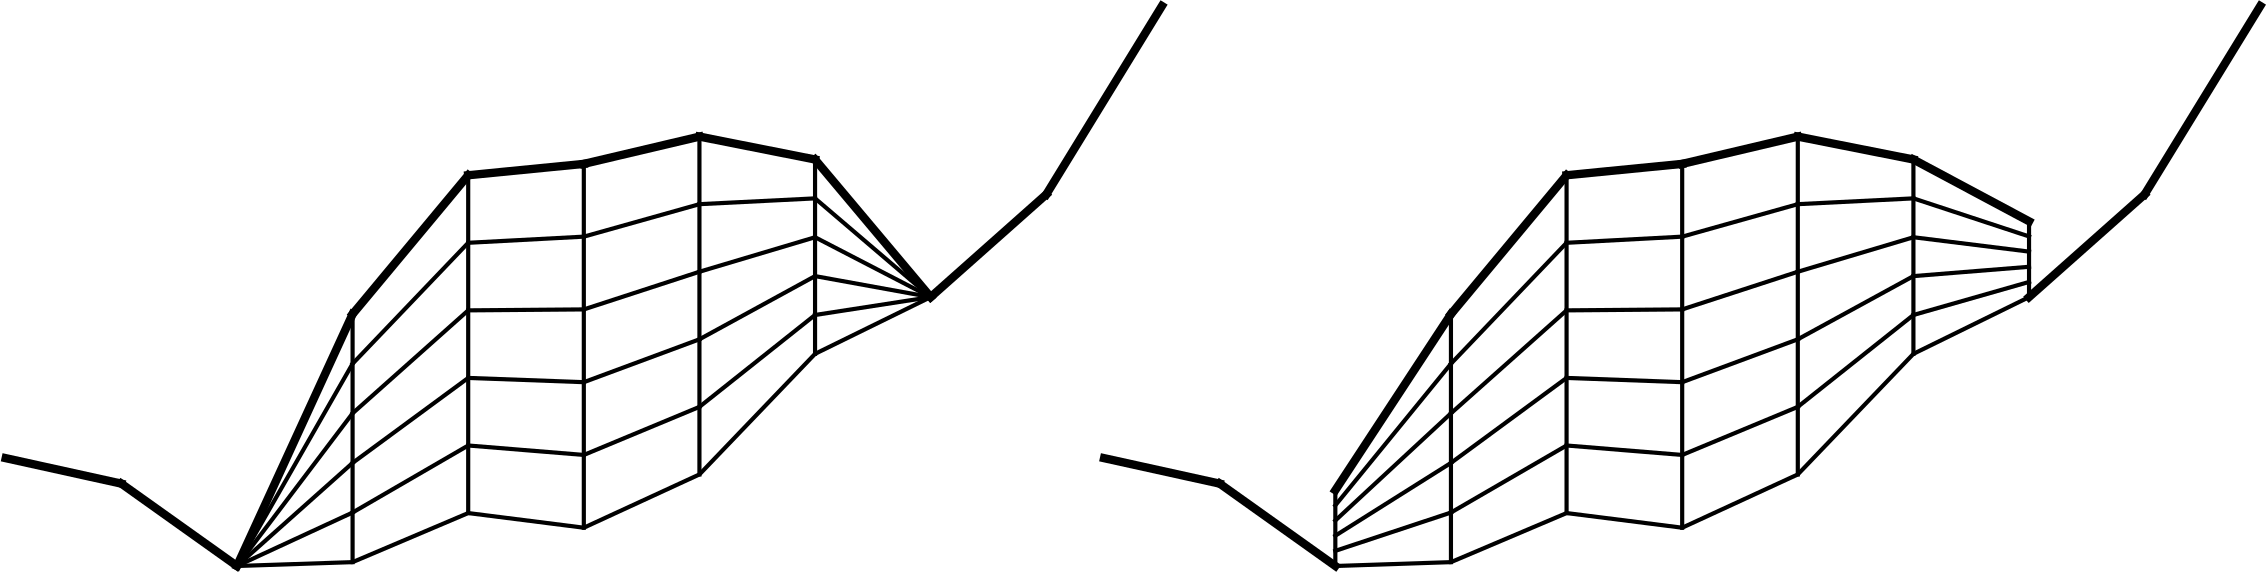
\includegraphics[width=\textwidth]{genfigs/extruded.pdf}
\end{center}
\caption{We compute the IDO $\Phi^h(s^h)$ by solving \eqref{eq:glenstokesweak} on an extruded mesh with $m_z$ layers.  In the ``pinched'' extrusion (left), the trace of $\bu^h$ is evaluated on the graph of $s^h$ (bold).  In the ``cliffs'' extrusion (right) all elements have a minimum thickness so the trace evaluation may occur above $s^h$ (dotted).}
\label{fig:extruded}
\end{figure}

We will compare two extrusion modes.  In the ``pinched'' extrusion the elements cover $\Lambda_{s^h}$ exactly.  It follows that the elements at the ice margin are degenerate; they have positive volume but zero height at some nodes or even empty (vertical) facets.  In the alternate ``cliffs'' extrusion, each extruded element is nondegenerate.  Specifically, each prism (quadilateral) element has minimum thickness $H_{\text{min}}/m_z$ where $H_{\text{min}} > 0$ is the minimum total thickness, with $H_{\text{min}} = 20$ meters in computations.  The surface $s^h$ remains unchanged (and continuous), so these cliffs are only relevent to problem \eqref{eq:glenstokesweak}.

Let $\Phi^h:\mathcal{K}^h \to (\mathcal{V}^h)'$ be the FE approximation of the IDO $\Phi$.  By definition $\Phi^h(s^h)$ is the normal component of the numerical surface velocity after solving the Glen-Stokes equation \eqref{eq:glenstokesweak} on the domain $\Lambda_{s^h}$.  That is, we evaluate $\Phi^h(s^h)$ using the surface trace as in \eqref{eq:ido}, and then extend by zero to all of $\Omega$.  In the ``cliffs'' extrusion the trace is computed at the top of each column, and thus not necessarily at the original surface $s^h$.

We solve the Glen-Stokes problem \eqref{eq:glenstokesweak} using a $P^2 \times P^1$ Taylor-Hood mixed space for $(\bu,p)$ \cite{Elmanetal2014}.  The power-law nonlinearity is resolved by using a Newton iteration, with direct solution of the step equations and back-tracking line search.  As stated in Section \ref{sec:intro}, our goal in the current paper is to show that $O(1)$ iterations of the multilevel scheme are needed to solve the SIGP \eqref{eq:sigpweakform}.  Overall optimality of the solution algorithm also requires an optimal solution of the Glen-Stokes problem, such as the multigrid scheme in \cite{IsaacStadlerGhattas2015}.

Finally, let $F^h(s)[r] = - \ip{\Phi^h(s)}{r}$; compare \eqref{eq:sigpfunctional}.  The discrete SIGP computes $s^h \in \mathcal{K}^h$ satisfying
\begin{equation}
F^h(s^h)[r^h - s^h] \ge \ip{a}{r^h-s^h} \quad \text{for all } r^h \in \mathcal{K}^h. \label{eq:fesigpweakform}
\end{equation}
The only role of the extruded mesh in solving \eqref{eq:fesigpweakform} is in the evaluation of the IDO $\Phi^h(s^h)$.  We believe that \eqref{eq:fesigpweakform} is well-posed, but this is subject to the same caveats in the last section regarding identification of Sobolev spaces, along with the concern about overhangs at the margin, and we have no proof.


\section{Smoothers} \label{sec:smoothers}

In this section we propose solvers for \eqref{eq:fesigpweakform}, namely certain projected and nonlinear iterations which are variants of the Gauss-Seidel and Jacobi methods, but made suitable for VIs \cite{KinderlehrerStampacchia1980}.  Given a current surface elevation $s^h\in \mathcal{K}^h$, these iterations sweep through the $m$ interior vertices ($P_1$ nodes) of $\mathcal{T}$ in a fixed order, solving one-dimensional VI problems.  While these iterations are adequate smoothers in a multilevel method (next section), they converge slowly if used as single-level methods.  Because of the non-locality and density of the IDO $\Phi^h$ (Section \ref{sec:weakido}), we must make careful approximations in order to retain adequate per-iteration performance.

Denote an arbitrary vertex of $\mathcal{T}$ by $(x_j,y_j)$ and let $\psi_j \in \mathcal{V}^h$ be the corresponding $P_1$ hat function, with $\psi_j(x_k,y_k)=\delta_{jk}$ \cite{Elmanetal2014}.  Let $\mathcal{W}_+^h = \{t^h \in \mathcal{V}^h \,:\, t^h \ge 0 \text{ and } t^h|_{\partial\Omega} = 0\}$.  Let $i=0,\dots,m-1$ index the interior vertices of $\mathcal{T}$, so $(x_i,y_i) \notin \partial\Omega$.  Note that $\psi_i \in \mathcal{W}_+^h$, and $s^h + c \psi_i \in \mathcal{K}^h$ if and only if $c\ge \beta_i^{s^h} = b^h(x_i,y_i) - s^h(x_i,y_i)$.  We call $\beta_i^{s^h}$ the pointwise defect obstacle \cite{GraeserKornhuber2009} for $s^h$.

The one-dimensional VI at interior node $i$ is derived from the discrete SIGP \eqref{eq:fesigpweakform} using $r = s^h+\gamma \psi_i$ and $s = s^h+c \psi_i$ for some scalars $\gamma,c$.  Specifically, we seek $c \ge \beta_i^{s^h}$ such that
\begin{equation}
F^h(s^h+c \psi_i)[(s^h+\gamma \psi_i) - (s^h+c \psi_i)] \ge \ip{a}{(s^h+\gamma \psi_i) - (s^h+c \psi_i)} \label{eq:fepointwiseviEARLY}
\end{equation}
for all $\gamma \ge \beta_i^{s^h}$.  Let
\begin{equation}
\rho_i(s^h; c) = F^h(s^h+c\psi_i)[\psi_i] - \ip{a}{\psi_i} \label{eq:ferhoi}
\end{equation}
be the point-wise residual function, and observe that \eqref{eq:fepointwiseviEARLY} simplifies to
\begin{equation}
(\gamma - c) \,\rho_i(s^h; c) \ge 0. \label{eq:fepointwisevi}
\end{equation}
The smoother will approximately solve \eqref{eq:fepointwisevi} for $c$ the smoother, and then update $s^h \gets s^h + c \psi_i$.  Observe that admissibility is preserved because $s^h+c \psi_i \in \mathcal{K}^h$ when $c \ge \beta_i^{s^h}$.

If $\rho_i(s^h; c)$ were linear and increasing in $c$, e.g.~$\rho_i(s^h; c) = \rho_i(s^h; 0) + \alpha c$ with $\alpha > 0$, then the solution to \eqref{eq:fepointwisevi} would be given by the simple formula $c = \max\left\{-\rho_i(s^h; 0)/\alpha, \beta_i^{s^h}\right\}$ \cite{GraeserKornhuber2009}.  In fact $\rho_i(s^h; c)$ is nonlinear, and we will linearize
\begin{equation}
\rho_i(s^h; c) \approx \rho_i(s^h; 0) + c\, \rho_i'(s^h; 0), \label{eq:rhoapprox}
\end{equation}
and at each node where $\rho_i'(s^h; 0) > 0$ we will do one projected Newton step using the simple formula.  If $\rho_i'(s^h; 0) \le 0$, so that the model has degenerated in the sense that the linearized, pointwise operator is not acting elliptically with respect to a perturbation, we set $c = \beta_i^{s^h}$ to remove the ice at that location.  % FIXME TOO AGGRESSIVE?

Because the interior PDE in the shallow, flat-bed model is elliptic, it follows that $\rho_i'(s^h; 0) > 0$ on the icy part of $\Omega$ \cite{JouvetBueler2012}.  However, for the full Glen-Stokes model there is no such guarantee to our knowledge.

Note that the derivative $\rho_i'(s^h; 0)$, which is also a diagonal entry of the Jacobian of $F^h$, can be approximated by a finite difference,
\begin{equation}
\rho_i'(s^h; 0) = (F^h)'(s^h)[\psi_i,\psi_i] \approx \frac{\rho_i(s^h; \eps) - \rho_i(s^h; 0)}{\eps}.  \label{eq:rhofd}
\end{equation}
Literal use of \eqref{eq:rhofd} is very expensive because each value $\rho_i(s^h; \eps)$ requires a separate Glen-Stokes computation for the residual.

If each pointwise update $s^h \gets s^h + c \psi_i$ is done immediately then the smoother is of Gauss-Seidel (GS) type, also called serial or multiplicative, while a (parallel, additive) Jacobi smoother computes and stores solutions $c$ at every node $i$ before doing any updates.  In linear problems GS generally converges in about half as many iterations \cite{Greenbaum1997}, but here a more glaring difference dominates, namely that GS imposes the expense of yet more residual evaluations.  Nonetheless, the GS iteration using a single Newton step and approximation \eqref{eq:rhofd} is a well-defined smoother, so we state it in Pseudocode \ref{pc:pngsslow}.  It is given in a form which also allows over-relaxation ($\id{omega} > 1$) or under-relaxation ($\id{omega} < 1$) if desired.  Note that the Glen-Stokes problem \eqref{eq:glenstokesweak} is solved $2m$ times per application of this function.

\begin{pcode}[ht]
\begin{pseudo*}
\pr{pngs\_slow}(s^h,b^h,\id{eps}=1.0,\id{omega}=1.0)\text{:} \\+
    \ct{check admissibility: $s^h \ge b^h$} \\
    for $i = 0,\dots,m-1$ \\+
        $\alpha_i = (\rho_i(s^h; \eps) - \rho_i(s^h; 0))/\eps$  \qquad\qquad \ct{Jacobian diagonal entry} \\
        if $\alpha_i > 0$ \\+
            $c_i = - \rho_i(s^h; 0) / \alpha_i$ \\
            $(s^h)_i \gets \max\{(s^h)_i + \id{omega}\,c_i, (b^h)_i\}$ \\-
        else \\+
            $(s^h)_i \gets \beta_i$ \qquad\qquad \ct{non-elliptic case}
\end{pseudo*}
\caption{Projected nonlinear GS iteration, an expensive in-place smoother using a finite-difference (FD) derivative for the Jacobian diagonal.}
\label{pc:pngsslow}
\end{pcode}

To build a better smoother we return to the computation of the Jacobian diagonal entry $\rho_i'(s^h; 0)$.  Suppose we partition the support of $\psi_i$ into where there is ice and not,
\begin{equation}
\theta_i = \{\psi_i > 0\} \cap \{s^h > b^h\}, \qquad {\hat\theta}_i = \{\psi_i > 0\} \setminus \theta_i.  \label{eq:thetasupport}
\end{equation}
Recall that $\bu|_{z}$ denotes the surface velocity of the solution to the Glen-Stokes problem \eqref{eq:glenstokesweak} on the domain $\Lambda_{z}$, using an extruded mesh (Section \ref{sec:fe}).  By \eqref{eq:idoderiv}, \eqref{eq:differencecases}, and \eqref{eq:ferhoi} we may compute
\begin{equation}
\rho_i(s^h; 0) = F^h(s^h)[\psi_i] - \ip{a}{\psi_i} = - \int_{\theta_i} (\bu|_{s^h} \cdot \bn_{s^h}- a)\, \psi_i  \label{eq:rhozero}
\end{equation}
and
\begin{align}
\rho_i'(s^h; 0) &= (F^h)'(s^h)[\psi_i,\psi_i]  \label{eq:rholocalderiv} \\
  &= - \int_{\theta_i} \lim_{\eps\to 0^+} \frac{(\bu|_{s^h+\eps\psi_i} - \bu|_{s^h}) \cdot \bn_{s^h+\eps\psi_i}}{\eps} \psi_i - \int_{{\hat\theta}_i} \lim_{\eps\to 0^+} \frac{\bu|_{s^h+\eps\psi_i} \cdot \bn_{s^h+\eps\psi_i}}{\eps} \psi_i.  \notag
\end{align}

Clearly, any smoother application, which is a sweep over all nodes in $\mathcal{T}$, will require at least one Glen-Stokes velocity solution, namely from solving \eqref{eq:glenstokesweak} on the geometry determined by the current surface elevation $s^h$.  Formulas \eqref{eq:rhozero} and \eqref{eq:rholocalderiv} as stated require a Stokes solution $\bu|_{s^h+\eps\psi_i}$ for each mesh node.

However, we may estimate the surface velocity for a such perturbed surface elevation, namely with a small ``bump'' $\eps\psi_i$, by replacing the geometrical bump with a local perturbation of the body force.  That is, we may perturb the gravitational load relative to the solution which gave $s^h$, but without changing the geometry.  The change to the nonlinearities in this Glen-Stokes problem should be small, and the most important change to the velocity and pressure fields from a small bump perturbation is through its weight.  We suppose that other effects, such as a perturbed normal direction on the surface, are significantly smaller.

FIXME Let us fix a current surface elevation $s^h$ and assume that problem \eqref{eq:glenstokesweak} for $\Lambda_{s^h}$ yields solution $\bu^h,p^h$ at the convergence of its (Newton) iteration.  Noting that we are using a stable mixed space for this Glen-Stokes problem (Section \ref{sec:fe}), the final step in the iteration can be regarded as providing the solution of a linear system
\begin{equation}
    \begin{bmatrix} A & B^\top \\
                    B & 0      \end{bmatrix}
    \begin{bmatrix} \bu^h \\ p^h \end{bmatrix}
    = \begin{bmatrix} \rhoi \bg \\ 0 \end{bmatrix}.  \label{eq:system}
\end{equation}
where we note that the matrix depends on $s^h$.  (Even the size of $K$ depends on $s^h$ because it is used to determine which $T\in\mathcal{T}$ get extruded icy columns.)  Also denote the perturbed problem, for surface $s^h + \eps \psi_i$, using an $\eps$ subscript.

We assert that the perturbed-geometry Glen-Stokes solution is approximated by re-using the unperturbed matrix but adding the mass of the bump $\eps \psi_i$ to the right-hand side:
\begin{equation}
\begin{bmatrix} A_\eps & B_\eps^\top \\
                B_\eps & 0      \end{bmatrix}
\begin{bmatrix} \bu_\eps^h \\ p_\eps^h \end{bmatrix}
    = \begin{bmatrix} \rhoi \bg \\ 0 \end{bmatrix}
\qquad \approx \qquad
\begin{bmatrix} A & B^\top \\
                B & 0      \end{bmatrix}
\begin{bmatrix} \bu_\eps^h \\ p_\eps^h \end{bmatrix}
    = \begin{bmatrix}  \rhoi (1 + \eps \tau_i)\bg  \\ 0 \end{bmatrix}.  \label{eq:systemmassanalogy}
\end{equation}
Here $\tau_i$ is a positive $P_1$ function on $\Lambda_{s^h}$, that is, on the extruded $d+1$-dimensional mesh, with support only at the top-surface node with base mesh index $i$, and with magnitude such that if $\eps=1$ meter then
\begin{equation}
  \int_{\Lambda_{s^h}} \tau_i\,dx\,dy\,dz = \int_\Omega \psi_i\,dx\,dy . \label{eq:massanalogy}
\end{equation}
In words, we approximate the Glen-Stokes solution $\bu_\eps^h,p_\eps^h$ for the perturbed geometry by re-using the same (i.e.~$s^h$) geometry but solving the final linear system using a right-hand-side perturbation of the equivalent mass to the geometry perturbation.  This is shown in Figure \ref{fig:massanalogy}.

\begin{figure}[t]
\begin{center}
FIXME %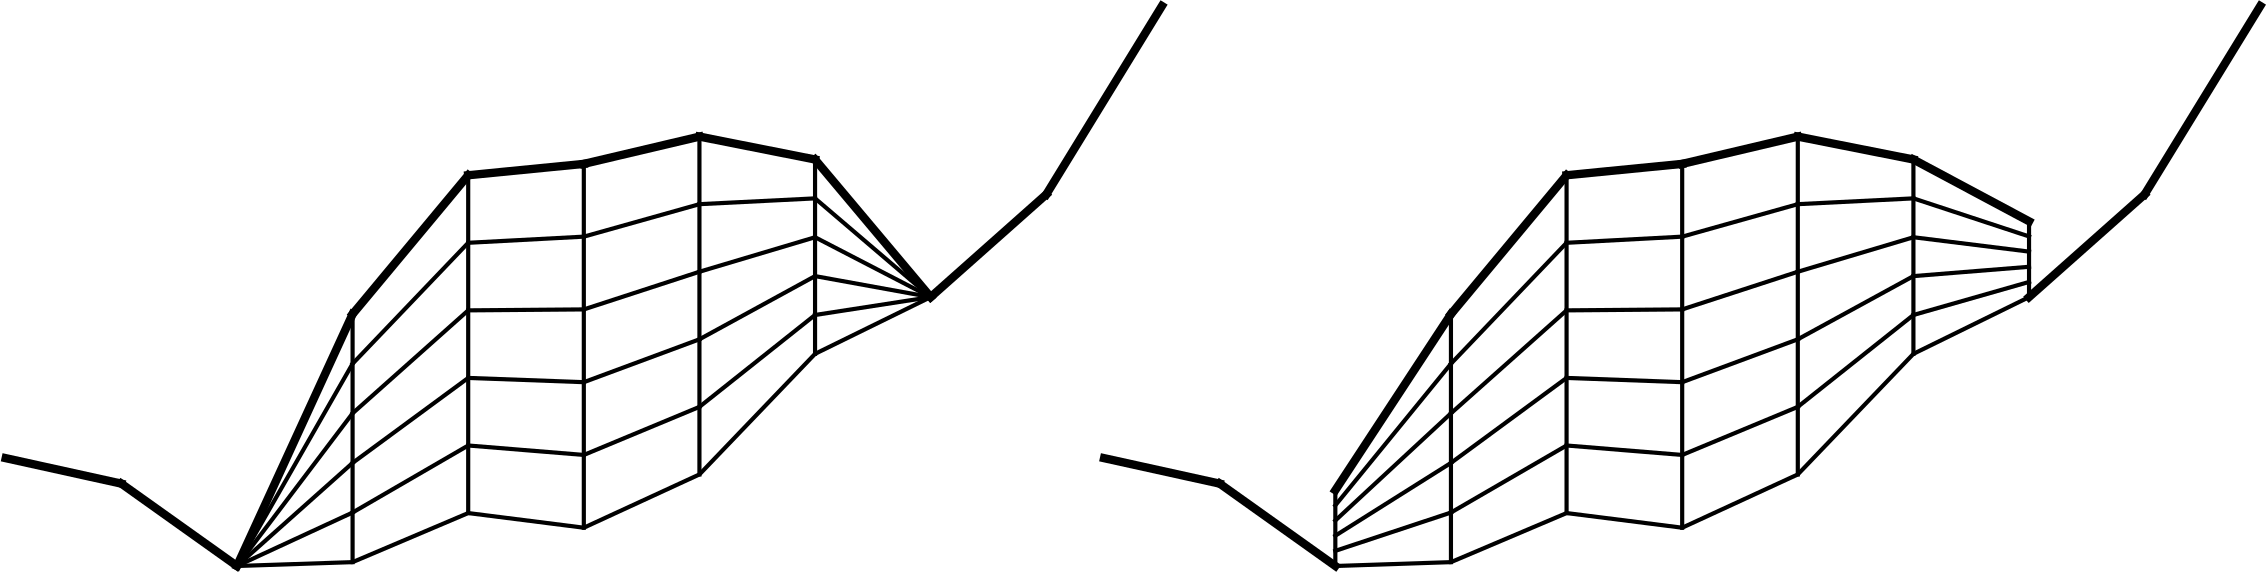
\includegraphics[width=\textwidth]{genfigs/extruded.pdf}
\end{center}
\caption{A sketch of the mass-perturbation approximation in equations \eqref{eq:systemmassanalogy} and \eqref{eq:massanalogy}.}
\label{fig:massanalogy}
\end{figure}

FIXME Pseudocode \ref{pc:pnj} for PNJ with bump approximation

\begin{pcode}[ht]
\begin{pseudo*}
\pr{pnj}(s^h,b^h,\id{omega}=1.0)\text{:} \\+
    \ct{check admissibility: $s^h \ge b^h$} \\
    evaluate $\{\rho_i(s^h; 0)\}_{i=0}^{m-1}$  \qquad\qquad \ct{and save the final Newton step linear system} \\
    for $i = 0,\dots,m-1$ \\+
        $\alpha_i = (A^{-1})_{ii}$  \qquad\qquad \ct{FIXME: give correct Jacobian diagonal entry} \\
        if $\alpha_i > 0$ \\+
            $c_i = - \rho_i(s^h; 0) / \alpha_i$ \\--
    for $i = 0,\dots,m-1$ \\+
        if $\alpha_i > 0$ \\+
            $(s^h)_i \gets \max\{(s^h)_i + \id{omega}\,c_i, (b^h)_i\}$ \\-
        else \\+
            $(s^h)_i \gets \beta_i$ \qquad\qquad \ct{non-elliptic case}
\end{pseudo*}
\caption{Projected nonlinear Jacobi smoother using a bump approximation for the Jacobian diagonal entry $\alpha_i$.  Problem \eqref{eq:glenstokesweak} is solved only once per application of \pr{pnj}, but additional linear algebra is needed to compute $\alpha_i$.}
\label{pc:pnj}
\end{pcode}

We finish this section with some observations which are supported by the results reported in Section \ref{sec:results}.  Constructing an efficient smoother is the most difficult part of building an effective multilevel scheme for numerically solving the SIGP.  In the time-stepping approach to steady state, used by almost all existing models, the difficulty is reflected in the nontrivial determination of a valid conditionally-stable time step criterion for the evolving geometry model.  Here the concern is associated to the ``ellipticity'' of the coupled equations for the SIGP, reflected in whether the diagonal Jacobian entry $\alpha_i$, used in the above pointwise smoothers, is indeed positive.

In fact, suppose $s^h$ gives the $P_1$ geometry of the ice which solves the discrete SIGP.  For each icy node $i$ in $\Omega$, i.e.~such that $(s^h)_i>(b^h)_i$, one can see that $\alpha_i>0$ if and only if the addition of a thin (e.g.~one meter) layer of ice to surface of the ice, covering the vicinity of node $i$ (e.g.~the support of $\psi_i$) will cause a dynamical response in which the surface goes down.  One can show this is so for the SIA theory \cite{JouvetBueler2012}, but, even for nonsliding ice, we know of no proof that the Glen-Stokes SIGP always gives $\alpha_i>0$ at icy locations.  It follows that pointwise smoothers like \pr{pngs\_slow} and \pr{pnj} are inherently fragile across a full range of glacier geometries.

FIXME SMOOTHER POSSIBILITIES.  1 COLORING (PSEUDO-COLORING WITH LATERAL SEPARATION OF A FEW ICE THICKNESSES).  2 PATCH-TYPE WHICH SOLVE LOW-DIMENSIONAL VI.


\section{Multilevel constraint decomposition} \label{sec:mcdstokes}

In this section we propose a new multilevel scheme for solving the discrete SIGP weak form \eqref{eq:fesigpweakform} using iterated V-cycles.  The fundamental idea of such a scheme is the basic geometric multigrid idea that smoothing on coarse levels will rapidly reduce the high frequencies in the error, but here we must maintain admissibility on each level in a manner which does not re-introduce high frequencies.  Our method descends from the multilevel constraint decomposition (MCD) method of \cite{Tai2003}, see also \cite{GraeserKornhuber2009}, but our ``MCDN'' nonlinear variant uses a full approximation scheme (FAS) multigrid \cite{Trottenbergetal2001} approach which transfers both the current residual and an approximation of the solution down to coarser levels.

Regarding notation for multiple mesh levels, suppose $\mathcal{T}^0$ is a fixed triangulation of $\Omega$, the coarse level.  For $J\ge 0$, suppose $\{\mathcal{T}^j\}_{j=1}^J$ are standard uniform refinements of $\mathcal{T}^0$ by edge bisection so that each $T \in \mathcal{T}^j$ becomes four similar triangles in $\mathcal{T}^{j+1}$ \cite{Braess2007}.  (Halve each interval when $d=1$.)  Let $\mathcal{V}^j$ be the $P_1$ FE space on $\mathcal{T}^j$, with subspace $\mathcal{V}_0^j \subset \mathcal{V}^j$ which are zero on $\partial\Omega$.  If $m_j$ is the number of interior nodes $\{(x_i^j,y_i^j)\}$ in $\mathcal{T}$ then $\dim(\mathcal{V}_0^j)=m_j$.  We seek an admissible solution to \eqref{eq:fesigpweakform} on the fine level $\mathcal{T}^J$.  Suppose $b^J \in \mathcal{V}^J$ denotes the fine-level bed topography.  The admissible surface elevations form a closed and convex set
\begin{equation}
\mathcal{K}^J = \{r^J \in \mathcal{V}^J \,:\, r^J \ge b^J, r^J|_{\partial\Omega} = b^J|_{\partial\Omega}\}.  \label{eq:singleadmissible}
\end{equation}

However, we follow \cite{GraeserKornhuber2009} in decomposing a ``defect obstacle'' formulation, and not direct use of the set $\mathcal{K}^J$.  That is, suppose $s^J \in \mathcal{K}^J$ is an admissible current iterate and let
\begin{equation}
\chi^J = b^J - s^J \in \mathcal{V}_0^J \label{eq:finedefectobstacle}
\end{equation}
be the associated defect obstacle, with $\chi^J \le 0$.  Note that $z^J \in \mathcal{V}_0^J$ is an admissible perturbation of $s^J$, i.e.~$s^J+z^J \in \mathcal{K}^J$, if and only if $z^J \ge \chi^J$.  Suppose $z^j \in \mathcal{V}_0^j$ is expanded in interior-node hat functions $\psi_i^j$, and define the monotone restriction operator $\mR : \mathcal{V}_0^j \to \mathcal{V}_0^{j-1}$ \cite{GraeserKornhuber2009} on $z^j = \sum_{i=0}^{m_j-1} z^j[i] \psi_i^j$ by maximizing nodal values over the (open) supports of each each coarser-level hat function:
\begin{equation}
\mR z^j = \sum_{\ell=0}^{m_{j-1}-1} \max\left\{z^j[i] \,:\,\psi_\ell^{j-1}(x_i^j,y_i^j) \right\}\,\psi_\ell^{j-1}.  \label{eq:monotonerestriction}
\end{equation}
Using $\mR$ a defect obstacle is defined on each level:
\begin{equation}
\chi^{j-1} = \mR \chi^j  \label{eq:recursivedefectobstacle}
\end{equation}
for $j=1,\dots,J$.  An example is shown in Figure \ref{fig:decompclassical}.  We also compute the differences,
\begin{equation}
\phi^j = \chi^j - \chi^{j-1},  \label{eq:downobstacles}
\end{equation}
with $\phi^0=\chi^0$ by definition; note $\phi^j\le 0$.

% figure generated in mg-glaciers/py by using decomposition_plain() in visualize.py and then:
% $ ./obstacle.py -J 5 -jcoarse 1 -irtol 1.0e-5 -monitor -diagnostics -random -randommodes 15 -o classical.pdf
% to get decomp_classical.pdf
\begin{figure}[t]
\begin{center}
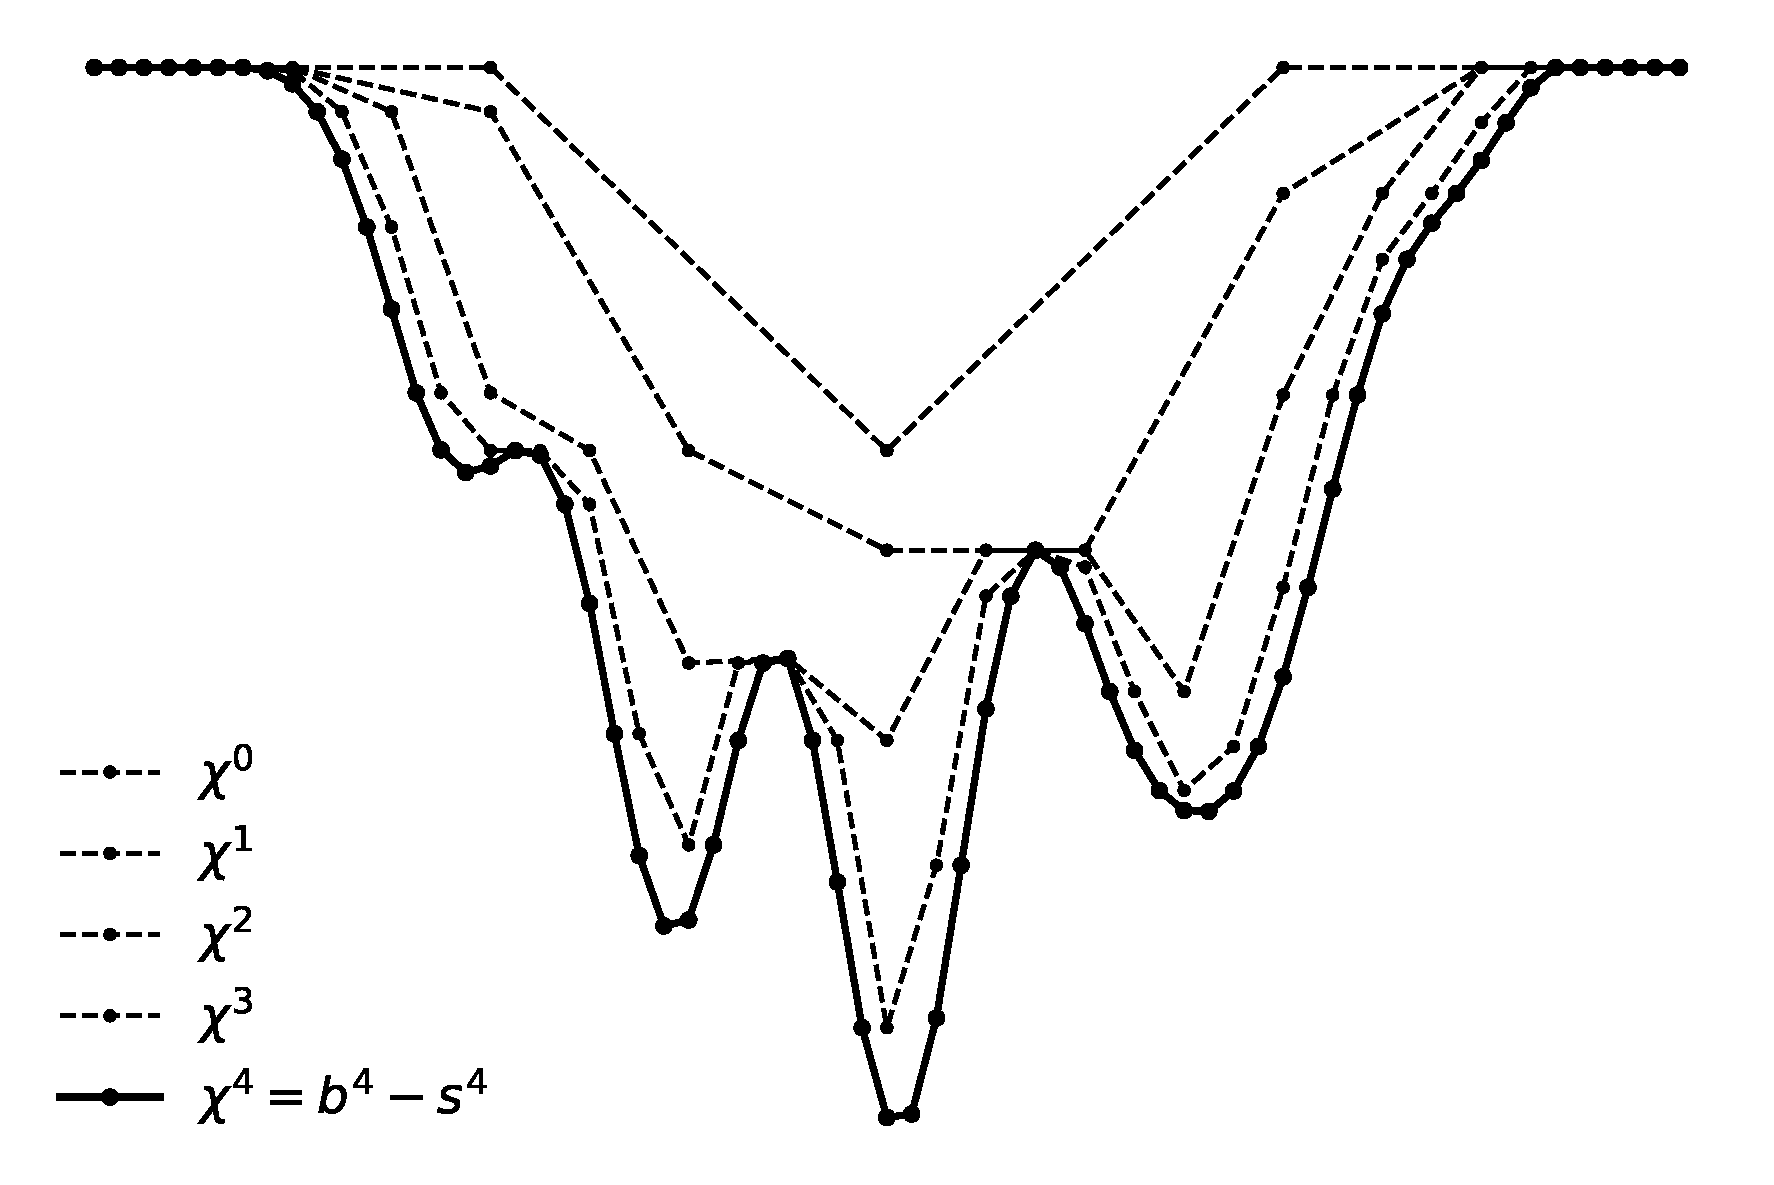
\includegraphics[width=0.7\textwidth]{fixfigs/decompclassical.pdf}
\end{center}
\caption{An example ($d=1$, $J=4$) of an MCD decomposition of the defect obstacle $\chi^J$.  Defect obstacles $\chi^j$ are generated using the monotone restriction operator $\mR$ as in \eqref{eq:recursivedefectobstacle}.}
\label{fig:decompclassical}
\end{figure}

A point-wise smoother on a given level will solve one-dimensional VIs at each node.  However, different admissible sets are used going down and up in the V-cycle.  Let
\begin{equation}
\mathcal{D}^j = \left\{y^j \in \mathcal{V}_0^j \,:\, y^j \ge \phi^j\right\}, \qquad \mathcal{U}^j = \left\{z^j \in \mathcal{V}_0^j \,:\, z^j \ge \chi^j\right\}. \label{eq:downupsets}
\end{equation}
The down-admissible constraint sets $\mathcal{D}^j$ sum to an up-admissible constraint set for each level, i.e.~$\mathcal{D}^0 + \mathcal{D}^1 + \dots + \mathcal{D}^j = \mathcal{U}^j$ in the sense that every $z^j \in \mathcal{U}^j$ is the sum of elements, though not uniquely.  The $\mathcal{U}^j$ are themselves nested in $\mathcal{U}^J= \{z^J \,:\, z^J \ge b^J - s^J\}$, and this forms a multilevel cone approximation, from the inside, of the continuum defect constraint set $\mathcal{K} - s = \{z\,:\,z \ge b - s\}$:
\begin{equation}
\mathcal{U}^0 \subset \mathcal{U}^1 \subset \dots \subset \mathcal{U}^J \subset \mathcal{K} - s \subset W_0^{1,\qq}(\Omega). \label{eq:innerconeapprox}
\end{equation}

We seek a solution to VI \eqref{eq:fesigpweakform} on the fine level.  The original idea of Tai \cite{Tai2003} is to use a multilevel constraint decomposition (MCD) like the above  system $\{\mathcal{D}^j\}$ to compute corrections $y^j \in \mathcal{D}^j$ which sum to a solution of the (nonlinear) fine-level VI,
\begin{equation}
F^J(s^J + y^J + \dots + y^j)[v^j - y^j] \ge (a,v^j - y^j) \quad \text{for all } v^j \in \mathcal{D}^j, \label{eq:mcdoriginal}
\end{equation}
where $F^J = F^h$ in \eqref{eq:fesigpweakform}.  In \cite{Tai2003}, VIs \eqref{eq:mcdoriginal} are to be solved on descending levels $j=J$ down to $j=0$, forming a down-slash or V(1,0) cycle.  (See also \cite[Algorithm 4.7]{GraeserKornhuber2009}.)  Note that $y^J + \dots + y^j \in \mathcal{U}^J$ so $s^J + y^J + \dots + y^j \ge b^J$ is admissible in the original sense, and that \eqref{eq:mcdoriginal} exploits the simplification $(s^J + y^J + \dots + v^j) - (s^J + y^J + \dots + y^j) = v^j - y^j$.

However, there is no practical way to achieve rapid solution of VI \eqref{eq:mcdoriginal} on coarse levels if the latest iterate $s^J + y^J + \dots + y^j$ must be represented; it has fine-level content.  This is the reason to add the full approximation scheme (FAS) \cite{Trottenbergetal2001} concept of a nonlinear coarse-level ``equation'', which is here a nonlinear VI.  In order to implement our approach we need to state the FAS coarse-level correction equation based on appropriate restrictions, as follows.

Let $\iR: \mathcal{V}^{j+1} \to \mathcal{V}^j$ be the injection restriction operator \cite{Trottenbergetal2001}.  Suppose $y^j \in \mathcal{D}^j$ denotes the desired down-correction on the $j$th level.  For corrections $y^j \in \mathcal{D}^j$, define $t^j \in \mathcal{V}^j$ as the $j$th-level approximation to the corrected fine-level solution (i.e.~$t^j \approx s^J + y^J + \dots + y^j$),
\begin{equation}
t^j = \begin{cases} s^J, & j=J \\
                    \iR(t^{j+1} + y^{j+1}), & j < J.
      \end{cases}  \label{eq:fassolution}
\end{equation}
Note that $t^j$ satisfies $t^j \ge \iR(\dots(\iR(b^J))\dots)$ by construction because $y^j \in \mathcal{D}^j$.  Though represented on a coarse level, $t^j$ has admissible point values relative to the fine bed $b^J$.

Let $F^j$ represent the FE discretization of $F$ (Section \ref{sec:fe}) on the $j$th level, and let $R: (\mathcal{V}^{j+1})^* \to (\mathcal{V}^j)^*$ be the canonical restriction on functionals \cite{GraeserKornhuber2009}.  The FAS coarse-level VI is
\begin{equation}
F^j(t^j+y^j)[v^j-y^j] \ge \ell^j[v^j-y^j] \quad \text{for all } v^j \in \mathcal{D}^j. \label{eq:fasequation}
\end{equation}
where
\begin{equation}
\ell^j[v] = \begin{cases} \ip{a}{v}, & j=J \\
                          F^j(t^j)[v] + R \left(\ell^{j+1} - F^{j+1}(t^{j+1}+y^{j+1})\right)[v], & j < J. \end{cases}  \label{eq:fasell}
\end{equation}
On the one hand, all quantities in VI \eqref{eq:fasequation} are represented on the $j$th level, without reference to finer-mesh data.  On the other hand, for $j<J$ the VI \eqref{eq:fasequation} can be rearranged using \eqref{eq:fasell} to a correction form like the FAS equation for PDEs (e.g.~\cite[equation (5.3.12)]{Trottenbergetal2001}),
\begin{equation}
F^j(t^j+y^j)[v^j-y^j] - F^j(t^j)[v^j-y^j] \ge R \left(\ell^{j+1} - F^{j+1}(t^{j+1}+y^{j+1})\right)[v^j-y^j], \label{eq:fasequationtraditional}
\end{equation}
for all $v^j \in \mathcal{D}^j$.  In \eqref{eq:fasequationtraditional} the functional on the left and right side should be smooth, thus explaining \eqref{eq:fasequation}.  Following the solution of \eqref{eq:fasequation} on all descending levels $j=J,\dots,0$, in fact done by a smoother on each level, a V(1,0) cycle is completed and the new fine-mesh iterate is $s^J + y^J + \dots + y^0$.

The above formulas suffice for a V(1,0) cycle, and represent the FAS extension of Algorithm 4.7 in \cite{GraeserKornhuber2009}, and of the method of Tai \cite{Tai2003}.  However, for better performance we note that on the ascending part of a V-cycle we can smooth in a less-constrained set, the larger set $\mathcal{U}^j \supset \mathcal{D}^j$.  Regarding admissibility, the difference between descending and ascending in a V-cycle is that in the former case there are yet-to-be-computed corrections which we must force into small-enough sets $\mathcal{D}^j$ so that their sum is still admissible.  When ascending we have already summed the coarser-level corrections so we can smooth the result in the larger, nested sets $\mathcal{U}^j$ without destroying the admissibility of the yet-finer corrections to come.

The above ideas define the following MCDN V-cycle Pseudocode \ref{pc:mcdn-vcycle}.  This algorithm calls a smoothers from Section \ref{sec:smoothers} and it uses the canonical prolongation $P:\mathcal{V}^j \to \mathcal{V}^{j+1}$.  The default settings correspond to a V(0,1) cycle which we have found to be most efficient in tests on the classical obstacle problem \cite{Bueler2022}.  The returned value is a correction to the current iterate $s^J$.

\begin{pcode}[ht]
\begin{pseudo*}
\pr{mcdn-vcycle}(J,s^J,b^J,\id{down}=0,\id{coarse}=1,\id{up}=1)\text{:} \\+
    $\chi^J, \,\ell^J, \,t^J = b^J - s^J, \,\ip{a}{\cdot}, \,s^J$ \\
    for $j=J$ downto $j=1$ \\+
      $\chi^{j-1} = \mR \chi^j$ \\
      $\phi^j = \chi^j - \chi^{j-1}$ \\
      $y^j = 0$ \\
      $\text{\pr{smoother}}^{\text{\id{down}}}(y^j,t^j,\ell^j,\phi^j)$ \qquad \qquad \ct{in $\mathcal{D}^j$} \\
      $t^{j-1} = \iR(t^j + y^j)$ \\
      $\ell^{j-1} = F^{j-1}(t^{j-1}) + R(\ell^j - F^j(t^j+y^j))$ \\-
    $y^0 = 0$ \\
    $\text{\pr{smoother}}^{\text{\id{coarse}}}(y^0,t^0,\ell^0,\chi^0)$ \qquad \qquad \ct{in $\mathcal{U}^0$} \\
    $z^0 = y^0$ \\
    for $j=1$ to $j=J$ \\+
      $z^j = P z^{j-1} + y^{j}$ \\
      $\text{\pr{smoother}}^{\text{\id{up}}}(z^j,t^j,\ell^j,\chi^j)$ \qquad \qquad \ct{in $\mathcal{U}^j$} \\-
    return $z^J$
\end{pseudo*}
\caption{MCDN V-cycle.}
\label{pc:mcdn-vcycle}
\end{pcode}

To our knowledge two aspects of this MCDN V-cycle are new:
\begin{enumerate}
\item While Tai \cite{Tai2003} defines and proves the convergence of a nonlinear MCD method, the implementation of this method cannot achieve $O(m_J)$ time for each V-cycle in nonlinear cases because the method refers to the fine level for the residual evaluation on each coarser level.  Our FAS-type modification achieve $O(m_J)$ time per V-cycle when applied to a local nonlinear problem, for example in the SIA model application in \cite{Bueler2022} in which the smoother is $O(m_j)$ on each level.  In our current Stokes case the smoother is nonlocal and $O(m_j)$ smoother time is not achieved.
\item Our V($\alpha$,$\beta$) cycles, with $\alpha$ down-smoother and $\beta$ up-smoother applications, are more efficient when $\beta >0$ than the method proposed in \cite{GraeserKornhuber2009} for $V(1,1)$ cycles because the smoothing occurs in a less-constrained set.
\end{enumerate}

Finally we consider when iterated V-cycles have converged.  For any discrete obstacle $\chi^j \in \mathcal{V}^j$, admissible iterate $z^j\in \{r^j \ge \chi^j\} \subset \mathcal{V}^j$, and residual vector $r^j \in (\mathcal{V}^j)'$ let
\begin{equation}
\vertiii{r^j}_{(z^j,\chi^j)} = \left(\sum_{z_i > \chi_i} |r^j[\psi_i^j]|^2 + \sum_{z_i = \chi_i} |\min\{r^j[\psi_i^j],0\}|^2\right)^{1/2}, \label{eq:cpnorm}
\end{equation}
where $\psi_i^j$ denotes a $j$th-level nodal basis function.  This defines a ``CP residual norm'' associated to the finite-dimensional complementarity problem $z^j \ge \chi^j$, $r^j(z^j) \ge 0$, and $(z^j-\chi^j) r^j(z^j) = 0$.  Note $z^j \in \mathcal{V}^j$ solves this CP if and only if $z^j$ is admissible and $\vertiii{r^j(z^j)}_{(z^j,\chi^j)}=0$.

As shown in Pseudocode \ref{pc:mcdn-solver}, we iterate MCDN V-cycles until the CP residual norm is small according to either an absolute or a relative tolerance.

\begin{pcode}[ht]
\begin{pseudo*}
\pr{mcdn-solver}(J,s^J,b^J,\id{atol}=10^{-20},\id{rtol}=10^{-3},\id{cyclemax}=100)\text{:} \\+
    $\rho_0=\vertiii{(a,\cdot) - F^J(s^J)[\cdot]}_{(s^J,b^J)}$ \\
    for $k=1,\dots,\id{cyclemax}$ \\+
        $s^J \gets s^J + \pr{mcdn-vcycle}(J,s^J,b^J)$ \\
        $\rho_k=\vertiii{(a,\cdot) - F^J(s^J)[\cdot]}_{(s^J,b^J)}$ \\
        if $\rho_k < \id{atol}$ or $\rho_k \le \id{rtol} \, \rho_0$ \\+
            break \\--
\end{pseudo*}
\caption{The SIGP is solved by iterating V-cycles (Pseudocode \ref{pc:mcdn-vcycle}) until the CP residual norm \eqref{eq:cpnorm} is small.}
\label{pc:mcdn-solver}
\end{pcode}


\section{Results for steady geometry} \label{sec:results}

FIXME in this paper the Glen-Stokes problem is solved by Newton linearization and (parallel) direct solution of the Newton step equations; Firedrake and PETSc \cite{Balayetal2020,Bueler2021} used to solve this dynamics problem and thereby evaluate the residual $F$; geometric multigrid schemes exist for the  Glen-Stokes problem \cite{IsaacStadlerGhattas2015}; see also \cite{BrownSmithAhmadia2013} and \cite{Tuminaroetal2016} which solve a first-order approximation of the Glen-Stokes ice sheet problem by geometric and algebraic multigrid, respectively

FIXME convergence results; scaling results


\section{Multilevel methods for evolving geometry} \label{sec:evolution}

FIXME time-dependent runs


\section*{Acknowledgments}  Thanks to David Maxwell for discussions regarding the formulation and well-posedness of the model.

\small

\bigskip
\bibliography{msg}
\bibliographystyle{siam}

\appendix

\section{Glossary of acronyms} \label{app:glossary}

\renewcommand{\arraystretch}{1.1}
\begin{longtable}{l|l|l}
\caption{Glossary of acronyms used in this paper.}
\label{tab:acronyms} \\ % \\ REQUIRED HERE
\toprule
\textbf{Acronym} {\Large$\strut$} & \textbf{Definition} & \textbf{Reference} \\ \hline
CMB & climatic mass balance & Section \ref{sec:stokesgeometry} \\
FAS & full approximation scheme & Section \ref{sec:mcdstokes} \\
FE & finite element & Section \ref{sec:fe} \\
GS & Gauss-Seidel & Section \ref{sec:smoothers} \\
IDO & ice dynamics operator & Section \ref{sec:weakido}, equation \eqref{eq:ido} \\
IIGP & implicit ice geometry problem & Section \ref{sec:evolution} \\
MCD & multilevel constraint decomposition & Section \ref{sec:mcdstokes} \\
MCDN & multilevel constraint decomposition (nonlinear) & Section \ref{sec:mcdstokes}, Pseudocode \ref{pc:mcdn-vcycle} \\
NCP & nonlinear complementarity problem & Section \ref{sec:stokesgeometry} \\
PNGS & projected, nonlinear Gauss-Seidel (smoother) & Section \ref{sec:smoothers}, Pseudocode \ref{pc:pngsslow} \\
PNJ & projected, nonlinear Jacobi (smoother) & Section \ref{sec:smoothers}, Pseudocode \ref{pc:pnj} \\
SIA & shallow ice approximation & Section \ref{sec:intro} \\
SIGP & steady ice geometry problem & Section \ref{sec:stokesgeometry}, equation \eqref{eq:strongform} \\
SKE & surface kinematical equation & Section \ref{sec:stokesgeometry}, equation \eqref{eq:ske} \\
VI & variational inequality & Section \ref{sec:weakido} \\
WU & work units & Section \ref{sec:mcdstokes} \\ % final \\ required
\bottomrule
\end{longtable}

\end{document}
